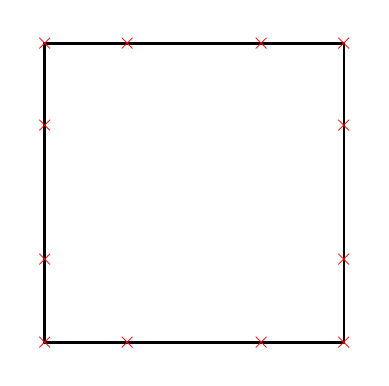
\begin{tikzpicture}
    \def\L{3.8}
    % 4-point Gauss--Lobatto positions in [0,1]:
    % (lambda+1)/2 for lambda in {-1, -0.4472, 0.4472, 1}
    \def\pa{0}
    \def\pb{0.2764}
    \def\pc{0.7236}
    \def\pd{1}

    % Cell boundary
    \draw[line width=0.9pt] (0,0) rectangle (\L,\L);

    % Bottom edge (y = 0): all 4 GL points
    \foreach \xi in {\pa, \pb, \pc, \pd}{
        \node[red, scale=0.85] at (\xi*\L, 0) {$\times$};
    }
    % Top edge (y = L): all 4 GL points
    \foreach \xi in {\pa, \pb, \pc, \pd}{
        \node[red, scale=0.85] at (\xi*\L, \L) {$\times$};
    }
    % Left edge (x = 0): interior 2 points only (corners already marked)
    \foreach \eta in {\pb, \pc}{
        \node[red, scale=0.85] at (0, \eta*\L) {$\times$};
    }
    % Right edge (x = L): interior 2 points only
    \foreach \eta in {\pb, \pc}{
        \node[red, scale=0.85] at (\L, \eta*\L) {$\times$};
    }
\end{tikzpicture}